% Chapter Template

\chapter{High-Dimension Model Representation Methods} % Main chapter title

\label{ch:methods hdmr} % Change X to a consecutive number; for referencing this chapter elsewhere, use \ref{ChapterX}

\lhead{Chapter 5. \emph{Methods: HDMR}} % Change X to a consecutive number; this is for the header on each page - perhaps a shortened title

%----------------------------------------------------------------------------------------
%	SECTION: INTRO
%----------------------------------------------------------------------------------------

\section{Introduction}\label{sec:hdmr intro}
As demonstrated in Chapter \ref{ch:results scgpc}, the Stochastic Collocation for generalized Polynomial Chaos
(SCgPC) methods for uncertainty quantification defined in Chapter \ref{ch:methods scgpc} can be very efficient
tools in comparison with traditional Monte Carlo to converge second-order statistics.  In particular, SCgPC
methods excel when the input dimensionality of a model is low and the response of interest is regular with respect
to the input space.  Conversely, they perform poorly with discontinuous responses and high dimensionality
input spaces.

Another useful model reduction method is High-Dimension Model Representation \cite{hdmr}, 
which is based on Sobol decomposition and is an ANalysis Of VAriance (ANOVA) method.  
ANOVA is a class of methodologies in statistics that seeks to determine the source of variances in a response
when considering the input space.  ANOVA methods originate in sampling statistics, where the structure of a
collection of samples is desired \cite{anova}.
The HDMR expansion helps
mitigate the problem of large input space dimensionality by dividing the model into a linear superposition of terms, 
each of which only depends on a subset of
the full input space.  The subsets are developed by integrating out the undesired dimensions.

Let $H(Y)$
represent the HDMR expansion of $u(Y)$,
\begin{equation}\label{eq:anova}
  u(Y) = H(Y) = h_0 + \sum_{n=1}^N h_n + \sum_{n_1=1}^N \sum_{n_2=1}^{n_1-1} h_{n_1,n_2} + \cdots +
  h_{1,2,\ldots,N},
\end{equation}
The $h_0$, the expected value, is given by
\begin{align}\label{eq:hdmr 0}
  h_0 &\equiv \int_{\Omega_1} \ldots\int_{\Omega_N} u(y_1,\ldots,y_N)\ dy_1\ldots\ dy_N, \\
    &= \int_\Omega u(Y) dY,
\end{align}
where $\Omega$ denotes the uncertainty space spanned by $Y$.
Recall also the definition of integration over the input space $\Omega$ given in Eq. \ref{eq: no rho}.  The first-order 
expansion terms $h_n$ are integrated as
\begin{equation}\label{eq:hdmr 1}
  h_n(y_n) \equiv \int_{\hat\Omega_n} u(Y)\ d\hat Y_n - h_0,
\end{equation}
where we use ``hat'' notation to refer to all elements except the one listed; for example,
\begin{equation}
  \hat Y_n \equiv (y_1,\cdots,y_{n-1},y_{n+1},\cdots,y_N),
\end{equation}
\begin{equation}
  \hat Y_{m,n} \equiv (y_1,\cdots,y_{m-1},y_{m+1},\cdots,y_{n-1},y_{n+1},\cdots,y_N).
\end{equation}
Similarly, $\hat\Omega$ is the slice of the input space only containing variables in $\hat Y$ and integration
over $\hat\Omega$ is weighted with respect to $\rho(\hat Y)$.
Second and higher-order HDMR expansion terms are defined as
\begin{equation}\label{eq:hdmr 2}
  h_{n_1,n_2}(y_{n_1},y_{n_2})) \equiv \int_{\hat\Omega_{n_1,n_2}} \hat\rho_{n_1,n_2}(\hat Y_{n_1,n_2}) u(Y)\
      d\hat Y_{n_1,n_2} - h_{n_1} - h_{n_2} - h_0,
\end{equation}
and so on.  Written another way, each subset is constructed by integrating over the domain with respect to all
input parameters the subset is not dependent on, then subtracting all other expansion subsets who depend on an
input space that is a subspace of the space on which the subset depends, including the expected value.
\begin{equation}
  h_{\vec s} = \int_{\hat\Omega_{\vec s}} u(Y)d\hat Y - \mlsum{s \subset \vec s\\|s|_1<|\vec s|_1}{} h_s,
\end{equation}
where $\vec s$ is a vector of dimensional ordinates with length less than or equal to the dimensionality $N$
of the input space.

There are many useful properties of this generic HDMR expansion.  First, each term represents the contribution
of that subset to the original response; that is, $h_1$ provides the contributions to the response solely
from variable $y_1$.  Further, the total contribution of a variable is the sum of all subsets for whom
variable is part of the subspace.  For example, the total contribution of $y_1$ to the response is the sum of
contributions from $h_1,h_{1,2},\cdots,h_{1,2,3}$, etc.

Second, full HDMR can easily be approximated by truncating terms from the expansion.  In particular, the
expansion can be limited to interactions between a finite number of variables.  Experience has shown
\cite{hdmrrabitz} that most of the high-order interaction terms are negligible.  The resulting truncated
expansion contains terms that are much lower-order than the original model, often without incurring
significant truncation error.  The full expansion requires many integrals to construct, often making it
inefficient when compared with using the original model.
Because the full expansion takes significant work to construct,
we assume some level of truncation is performed when using HDMR.

Third, the individual terms in the HDMR expansion are orthogonal with respect to the probability weight over
the input space; that is,
\begin{equation}
  \int_\Omega h_a h_b dY = 0 \hspace{10pt}\forall\hspace{5pt} a\neq b.
\end{equation}
Because of this, the second statistical moment of the HDMR expansion with respect to any subset dimension is
the equivalent to the second statistical moment of the associated subset,
\begin{equation}
  \int_{\Omega_n} H(Y)^2 dy_n = \int_{\Omega_n} h_n^2 dy_n.
\end{equation}
This in turn directly yields Sobol sensitivity coefficients.  Sobol sensitivity coefficients measure the impact on the
variance of a response as the result of changes in the variance of an input (or combination of inputs).  For
the HDMR expansion,
\begin{equation}
  \mathcal{S}_n \equiv \frac{\text{var}\qty[h_n]}{\text{var}\qty[H(Y)]},
\end{equation}
\begin{equation}
  \mathcal{S}_{m,n} \equiv \frac{\text{var}\qty[h_{m,n}]}{\text{var}\qty[H(Y)]},
\end{equation}
and so on.

\section{Cut-HDMR}\label{sec:cuthdmr}
The primary challenge in implementing HDMR for arbitrary responses is the integrals in Eq. \ref{eq:hdmr 0},
\ref{eq:hdmr 1}, and \ref{eq:hdmr 2}.  These integrals are of as high dimensionality as those required for
SCgPC.  As a result, at first glance HDMR seems to offer no benefits.  However,
we make use of an approximation for HDMR called \emph{cut-HDMR} \cite{cutHDMR} that makes a simplifying assumption.
In cut-HDMR, we assume the integral of a function over a dimension can be approximated by evaluating the
function at a set of reference values $\bar Y = (\bar y_1,\bar y_2,\cdots,\bar y_N)$, where bar notation
indicates the expected value of each input variable.  The reference value in this case
is a single point in the input space, often the mean of the input multidimensional probability distribution.  The
reference point, as well as planes and hyperplanes passing through the reference point, make up the
\emph{cuts} that give this method its name.  The cut-HDMR expansion $T(Y)$ of model $u(Y)$ is expressed as
\begin{equation}\label{eq:cuthdmr}
  u(Y) = T(Y) = t_r + \sum_{n=1}^N t_n + \sum_{n_1=1}^N \sum_{n_2=1}^{n_1-1}
  t_{n_1,n_2}+\cdots+t_{1,2,\ldots,N}.
\end{equation}
Eq. \ref{eq:cuthdmr} is identical in form to the traditional ANOVA HDMR expansion in Eq. \ref{eq:anova}, but the subset components
are defined differently,
\begin{equation}
  t_r \equiv u(\bar Y),
\end{equation}
\begin{equation}
  t_n(y_n) \equiv u(y_n,\barhat{Y_n}) - t_r,
\end{equation}
\begin{equation}
  t_{m,n}(y_m,y_n) \equiv u(y_m,y_n,\barhat{Y_{m,n}}) - t_m - t_n - t_r,
\end{equation}
and so on. Note that $\bar Y$ is the reference input realization, and 
$\barhat{Y_n}$ denotes a partial input realization where all inputs are at reference values and $y_n$ is
excluded:
\begin{equation}
  \barhat{Y_n} = (\bar y_1,\cdots,\bar y_{n-1},\bar y_{n+1},\cdots,\bar y_N).
\end{equation}
In the limit where each subset of cut-HDMR is at most linearly dependent on an input parameter, cut-HDMR and
ANOVA are identical and exact.  Additionally, both ANOVA and cut-HDMR converge exactly on the model if no
truncation is performed.

The immediate benefit from cut-HDMR is the ability to computationally calculate the terms in Eq.
\ref{eq:cuthdmr};
we only need the reference input realization $\bar Y$ to construct the expansion.  However, there are two
drawbacks to this expansion.  First, cut-HDMR approximates the expected value of a model as the value of the
model evaluated at the input parameters' expected value.  While higher-order expansion terms correct this
assumption, for low-order truncations it can have significant impact.
Second,
cut-HDMR component terms are not orthogonal, unlike standard HDMR (hereafter referred to as ANOVA to avoid
confusion).  This results in difficulty
when attempting to algorithmically determine statistical moments.  Fortunately, this will be resolved in
section \ref{sec:cut to anova}.  First, however, we consider how to represent the subset terms in the cut-HDMR
expansion in an algorithmically-efficient manner.

\section{gPC and cut-HDMR}\label{sec:gPC cut}
Consider the cut-HDMR expansion,
\begin{equation}
  u(Y) = T(Y) = t_r + \sum_{n=1}^N t_n + \sum_{n_1=1}^N \sum_{n_2=1}^{n_1-1}
  t_{n_1,n_2}+\cdots+t_{1,2,\ldots,N},
\end{equation}
with subsets $t$ defined in section \ref{sec:cuthdmr}. Each subset besides the reference solution $t_r$ is a
function of at least one uncertain input; for example, $t_1(y_1)$ and $t_{1,3,7}(y_1,y_3,y_7)$.  We can
consider each of these an independent uncertain model, with many of the same features as the entire model
$u(Y)$.  These subset terms have their own mean, variance, and sensitivities.  Additionally
these subsets can each be represented by a SCgPC expansion,
\begin{equation}
  t_n \approx \sum_{k'\in\Lambda'(L')} t_{n;k'}\Phi_{k'}(Y_n) - t_r,
\end{equation}
where we make use of prime notation $k'$, $\Lambda'$, $L'$ to denote a SCgPC expansion
for a subset term of a cut-HDMR expansion and $t_{n;k'}$ are the scalar expansion coefficients.  Eq.
\ref{eq:cuthdmr} can then be written
\begin{align}\label{eq:cut and gpc}
  T(Y) \approx t_r &+ \sum_{n=1}^N \qty(\sum_{k'\in\Lambda_n'(L')} t_{n;k'}\Phi_{k'}(Y_n)-t_r) \\ \nonumber
  &+ \sum_{n_1=1}^N \sum_{n_2=1}^{n_1-1} \qty(\sum_{k'\in\Lambda_{m,n}'(L')} t_{m,n;k'}\Phi_{k'}(Y_m,Y_n)
-t_m -t_n - t_r)\\
  \nonumber &+\cdots \\ \nonumber
  &+ \qty(\sum_{k'\in\Lambda_{1,\cdots,N}'(L')} t_{1,\cdots,N;k'}\Phi_{k'}(Y_1,\cdots,Y_N) - (\cdots)).
\end{align}

There are several synergies make available by using SCgPC to expand the subset terms in
the cut-HDMR expansion as in Eq. \ref{eq:cut and gpc}.  First, the scalar expansion coefficients can be calculated using the same
collocation-based methods developed for the SCgPC method.  
As we demonstrate in chapter \ref{ch:results scgpc},
these collocation methods are most efficient when the dimensionality is low and the response is smooth.
Because we expect the cut-HDMR expansion to be truncated at some finite level, consider the progression of the
terms retained in Eq. \ref{eq:cuthdmr}. The first term has zero dimensionality, the next set of terms all have
dimensionality of one, the next set two, and so forth.  All of the terms kept in cut-HDMR expansions
truncated to third-level interactions are dimensionality three or smaller, which is ideal size for
exceedingly efficient convergence of SCgPC methods.

In
addition, SCgPC methods are most efficient when the response is regular, or has a high degree
of continuity.  Whatever the
continuity of the original model, the continuity of the subsets in the HDMR expansion of that model are at
least as continuous, and can often be more continuous.  This is because the subsets are obtained by removing the 
dependence on some of the
constituent variables.  If any discontinuity in the original response is contributed by any of those variables,
the resulting continuity is greater for the subset.
Since cut-HDMR naturally divides up the subset space, it will
converge the smooth subsets rapidly, possibly converging on the original model more efficiently than purely
SCgPC can without using cut-HDMR for somewhat discontinuous responses.

Second, SCgPC polynomials are constructed to be inherently orthonormal.  As long as
consistency is maintained in the polynomial families between different cut-HDMR subsets, this orthonormality
extends into interactions between subsets.  We explore using this advantage to reconstruct ANOVA terms
in Appendix \ref{apx:cut anova}.

\section{On convergence of gPC and cut-HDMR with gPC}\label{sec:conv gpc hdmr}
We pause momentarily to make a note about the convergence of SCgPC
methods alone in contrast to using SCgPC as part of a cut-HDMR expansion.  There are two degrees of freedom in
defining static SCgPC expansion construction.
The first is the polynomial
construction strategy, such as hyperbolic cross, total degree, or tensor product, along with level of
anisotropy.  The second is the polynomial order limit $L$.  For cut-HDMR, however, in addition to the
polynomial set and level, we add another option: the HDMR truncation level.  The HDMR truncation level
determines the maximum dimensionality of any subset in the cut-HDMR expansion.  Equivalently, it determines
the order of interactions between variables to include in the expansion.  For instance, second-order HDMR
truncation limits the expansion to at most pairwise interactions.

Consider a cut-HDMR expansion that uses isotropic total degree polynomial index set construction strategy with
a limiting total polynomial order of $L$ for its subset gPC terms, and a comparable pure 
SCgPC expansion with the same isotropic total degree polynomial index set construction strategy and same
limiting total polynomial order $L$.  In this situation, cut-HDMR \emph{without truncation} is equivalent to
the SCgPC expansion.  Any truncation of the cut-HDMR yields an approximation to
the pure generalized polynomial expansion, and as mentioned in section \ref{sec:hdmr intro}, an untruncated
HDMR expansion is by nature
inefficient.  As a result, for a given polynomial order limit $L$, cut-HDMR can at
most match the convergence of the corresponding generalized polynomial chaos expansion.  Usually, it will be
less accurate than the SCgPC equivalent because of HDMR truncation error.  Additionally, the
full cut-HDMR expansion will use a very similar number of numerical evaluations to obtain an equal level of
convergence.  This means there is no improved efficiency for cut-HDMR over SCgPC.

However, the real benefit of cut-HDMR is seen in models with large input dimensionality.  In this case, even a
first-order SCgPC expansion using total degree index set construction could take
thousands of evaluations to construct.  Because cut-HDMR can be truncated to limited interactions, however,
for far fewer evaluations, cut-HDMR can be constructed.  For models that are computationally expensive and
thousands of solves are
prohibitive, the error incurred by truncating cut-HDMR may be worth the reduction in necessary evaluations.
Even though cut-HDMR might be less efficient, it may still be constructed when the SCgPC cannot.

\section{Reconstructing ANOVA from cut-HDMR}\label{sec:cut anova}
In general, it is not straightforward to calculate second-moment statistics of a cut-HDMR expansion, as the
subset terms are not orthogonal.  This means evaluating the integral of the product of every pair combination
of subsets in the expansion, which almost surely cannot be done analytically.
When using gPC to represent individual cut-HDMR subsets however, it is simple to analytically recover ANOVA statistics 
for a
cut-HDMR expansion, despite the lack of orthogonality in cut-HDMR terms.  This is because the gPC components
of each subset term are replete with orthogonal relationships.  Note that while this method will
obtain ANOVA results for cut-HDMR terms, the statistics gathered are for the cut-HDMR expansion, not for the
original model.  If the cut-HDMR expansion is truncated as expected, the ANOVA terms will only be as accurate
to the original model as the cut-HDMR expansion itself is.  

Ultimately, because of orthogonality, the variance contribution for each subset is the sum of the squares of all polynomial
coefficients whose associated polynomials are at least first-order polynomials with respect to all of the
subset's input space, and only the subset's input space.  The total variance is the sum of each subset's
variance contribution.

More discussion and an example of this process is provided in Appendix \ref{apx:cut anova}.

\section{Adaptive HDMR}
As discussed regarding the adaptive SCgPC method in section
\ref{sec:adaptive sparse grid}, it is not only possible but likely that different input variables have
different effective polynomial order impact on a response.  When constructing an HDMR expansion, we similarly
expect that often some subsets in the expansion will require fewer polynomials to represent well than others.
Often, however, an analyst
cannot know a priori to what order input subsets should be expanded to accurately represent a response
This is especially true when working with
abstract inputs such as those provided through a Karhunen-Leove expansion \cite{karhunen}.  As
with the adaptive SCgPC, it is convenient to have an
algorithmic adaptive HDMR expansion construction strategy.  Such an algorithm was proposed by Gerstner and Griebel
\cite{Gerstner} and demonstrated by Ayres and Eaton \cite{Ayres}.  The algorithm is used to determine which
subsets in the HDMR expansion should be included depending on what computational resources are available, in
an adaptive manner.  
We extend existing methodology to include
predictive algorithms for choosing forward directions.  Additionally, we consider an intermingled adaptive
approach of adaptive HDMR construction with adaptive sparse grid generalized polynomial chaos expansions for
subsets.  

\subsection{Adaptive Algorithm}
The existing algorithm \cite{Gerstner,Ayres} is expanded by considering both adaptive SCgPC and adaptive HDMR
acting simultaneously, as well as using predictive searching.
The algorithm proceeds as follows:
\begin{enumerate}
  \item Begin by constructing all the first-order HDMR subsets up to first-order polynomial expansions.
  \item While not converged:
    \begin{enumerate}
      \item Iterate through each existing HDMR subset and determine the estimated impact of adding the
        next-favored polynomial for that subsets SCgPC expansion.
      \item Determine the Sobol sensitivity coefficient for each HDMR subset using ANOVA (see Appendix
        \ref{apx:cut anova}).
      \item Predict the expected impact of adding each new eligible subset to the HDMR expansion.
      \item Compare the product of a polynomial impact and its subset Sobol sensitivity with the expected impact
        of the eligible subsets.
      \item Perform the most likely impactful operation (adding a new subset or adding a polynomial to an
        existing subset)
      \item Use the estimated impact of eligible HDMR subsets and eligible polynomials for each subset to
        estimate total truncation error (total of all SCgPC truncation errors as well as HDMR truncation error).
      \item Use previous iterations to approximate the convergence of the algorithm
      \item Combine estimated remaining variance with approximated convergence to determine convergence
      \item If convergence and estimated remaining variance are less than tolerance, convergence is reached.
      \item Otherwise, continue the algorithm.
    \end{enumerate}
\end{enumerate}
This process is diagrammed in Figure \ref{fig:ahdmr}.  Note that this diagram assumes there is a sample
submission process in a larger uncertainty quantification framework such as \raven{} \cite{raven}, which handles
computation resources in an efficient manner.  In the flow chart, green indicates initialization, purple
is the HDMR portion, blue is the SCgPC algorithms, yellow is the
convergence process, and red indicates successful exit.  Note that a path to the exit has been added for 
reaching some
user-defined maximum number of runs; this is useful for allowing the algorithm to perform a search using a
restricted amount of computational resources.
\begin{figure}[H]
  \centering
  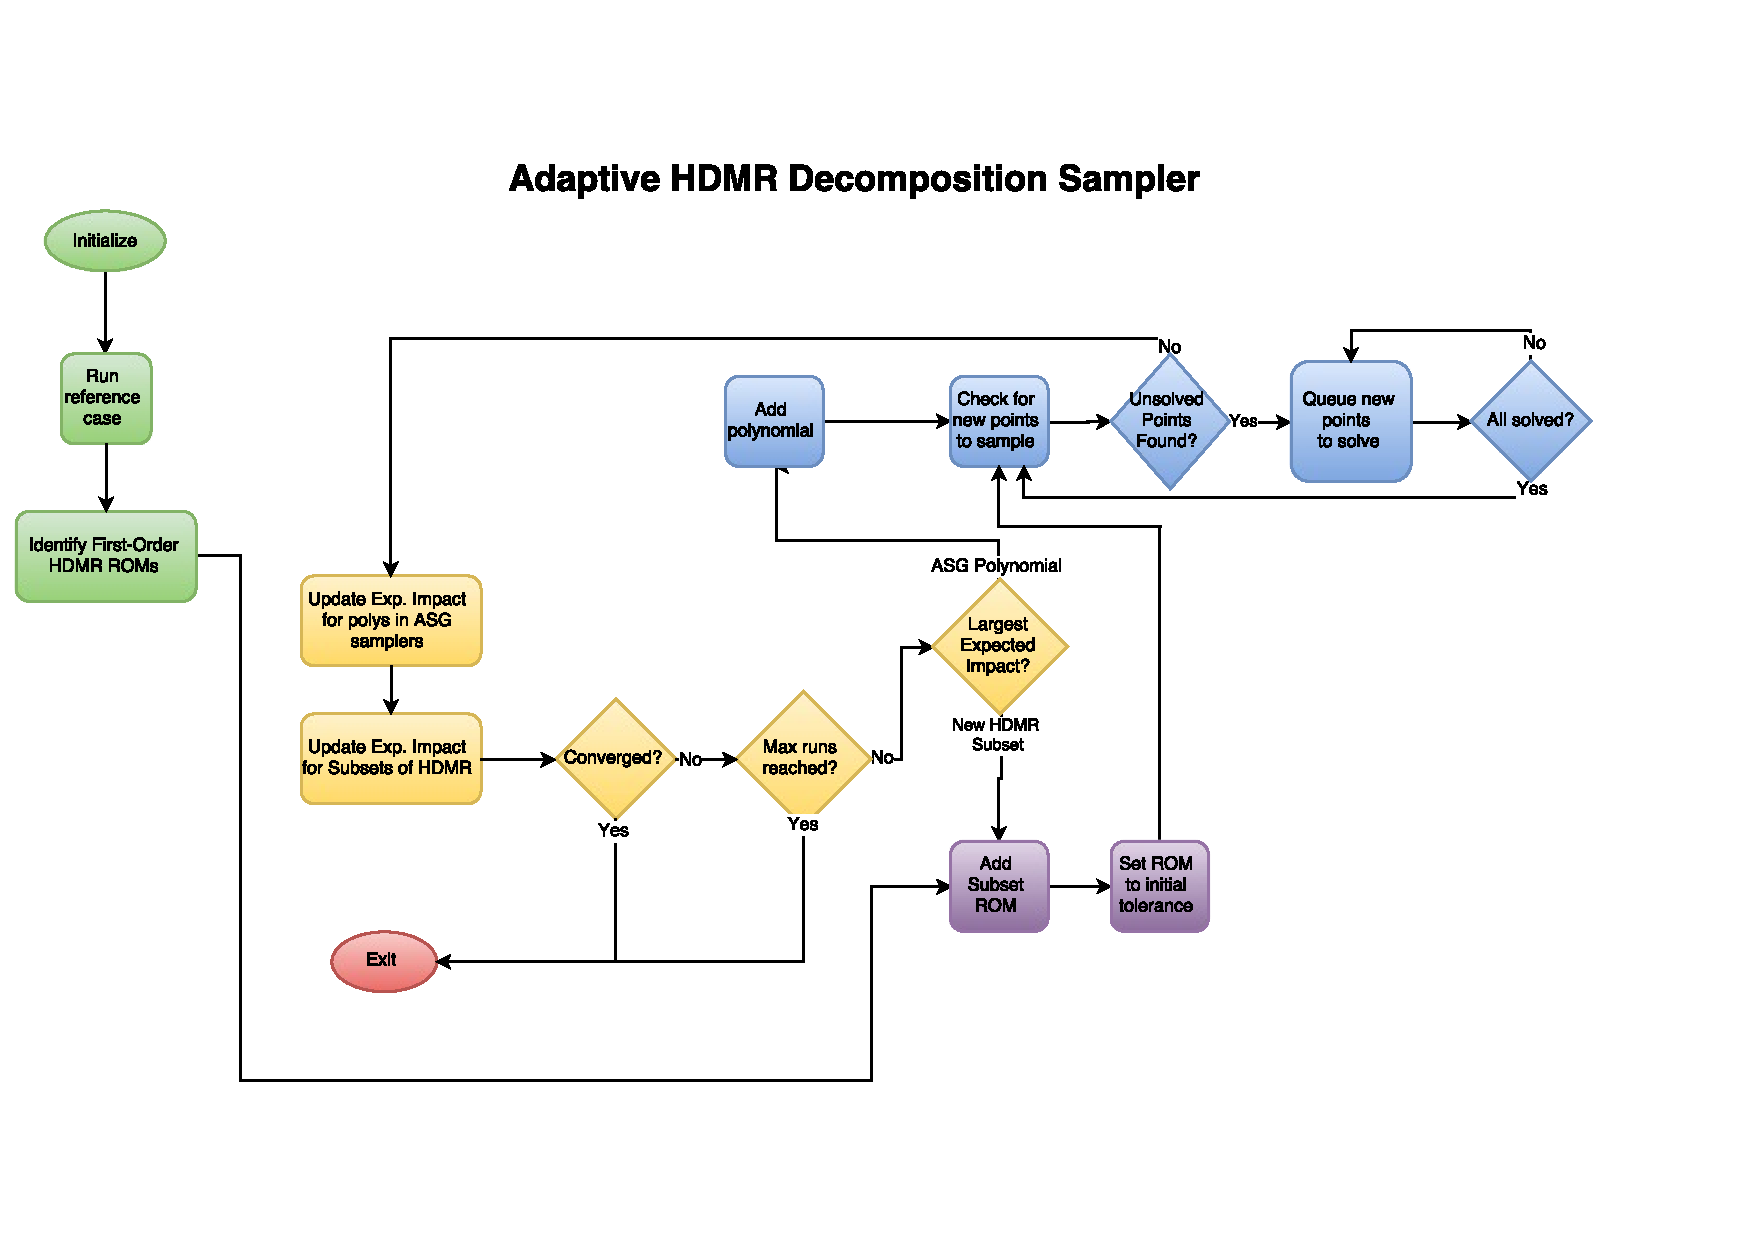
\includegraphics[width=\linewidth]{diagram-AHDMR}
  \caption{Adaptive HDMR with Adaptive Sparse Grid Flow Chart}
  \label{fig:ahdmr}
\end{figure}


Recall from section \ref{sec:adaptive sparse grid} that the impact of a polynomial within a subset generalized
polynomial chaos expansion is given by Eq. \ref{eq: poly impact},
\begin{equation}
  \tilde \eta_k = \frac{1}{N-j}\sum_{n=1}^N \eta_{k-e_n},
\end{equation}
where we omit a superscript $(y_n)$ to indicate the subset for which this polynomial is part of the SCgPC expansion.
As we discuss in section \ref{sec: one poly per subset}, we restrict each 
polynomial to be eligible for addition to only one HDMR subset apiece, making the distinction unnecessary.  
The Sobol sensitivities provide the (current) impact of an existing subset,
\begin{equation}
  S_\beta = \frac{\text{var}\qty[h_\beta]}{\text{var}\qty[T(Y)]},
\end{equation}
computing $h$ as described in appendix section \ref{sec:cut to anova}, and introducing subset descriptor $\beta$ which
can be any number and combination of input variables $y_n$ such that $\beta\subset Y$, or equivalently
$\beta\subset (y_1,\cdots,y_N)$.  

The estimated global impact $\tilde\xi_k$ of a
polynomial $k$ within a
subset $t_\beta$ is the product of its (estimated) local and (current) subset sensitivities,
\begin{equation}
  \tilde \xi_k = \tilde\eta_k\cdot S_\beta.
\end{equation}
Analogously, the actual global impact $\xi_k$ of a polynomial $k$ within a subset $t_\beta$ is the
product of its local and subset sensitivities,
\begin{equation}
  \xi_k = \eta_k\cdot S_\beta,
\end{equation}
with $\eta_k$ given in Eq. \ref{eq: act poly impact}.
The estimated impact $\tilde S_\beta$ of adding a new subset to the HDMR expansion is the average of its
dependent subsets' Sobol sensitivities,
\begin{equation}
  \tilde S_\beta = \frac{1}{\dim(\beta)}\hspace{-10pt} \mlsum{\gamma\subset\beta\\1+\dim(\gamma)=m}{}\hspace{-10pt} S_\gamma,
\end{equation}
where by $\dim(\beta)$ we denote the dimensionality of $\beta$.  For example,
\begin{equation}
  \tilde S_{y_1,y_2} = \frac{1}{2}\qty(S_{y_1}+S_{y_2}).
\end{equation}

The philosophy behind combining polynomial impact parameters and Sobol sensitivity parameters is to provide a
means to allow the adaptive algorithm to optimize computational resources.  In effect, taking the product of
the polynomial impact with the Sobol sensitivity provides a local-to-global contribution,
\begin{equation}
  \eta_k \cdot S_\beta = \xi_k,
\end{equation}
\begin{equation}
  \frac{\text{local contribution}}{\text{local variance}} \cdot \frac{\text{local variance}}{\text{global
        variance}} = \frac{\text{local contribution}}{\text{global variance}}.
\end{equation}
We consider momentarily the decision-making process of the adaptive algorithm.  There are four possible
comparisons the adaptive HDMR with adaptive SCgPC has to make: between polynomials within a HDMR subset,
between polynomials in different HDMR subsets, between potential new HDMR subsets, and between polynomials and
a potential new HDMR subset.  In each case, the algorithm must decide which modification to existing
expansions is most likely to contribute the largest to converging on second-order statistics.

Comparing polynomials within a subset is simple, and involves inquiring the truth of a statement like the
following:
\begin{equation}
  \tilde\eta_{k_1} \hspace{5pt}\stackrel{?}>\hspace{5pt} \tilde\eta_{k_2}.
\end{equation}
Similarly, comparing new subsets is straightforward,
\begin{equation}
  \tilde S_{\beta_1} \hspace{5pt}\stackrel{?}>\hspace{5pt} \tilde S_{\beta_2}.
\end{equation}
Comparing polynomials from different subsets requires only weighting them by their subset Sobol sensitivities,
\begin{equation}
  \tilde\eta_{k_1}S_{\beta_1} \hspace{5pt}\stackrel{?}>\hspace{5pt} \tilde\eta_{k_2}S_{\beta_2}.
\end{equation}
Comparing polynomials to subsets is somewhat more ambiguous,
\begin{equation}
  \tilde\eta_{k_1}S_{\beta_1} \hspace{5pt}\stackrel{?}>\hspace{5pt} \tilde S_{\beta_3}.
\end{equation}
Three cases can occur in comparing subsets to polynomials:
\begin{itemize}
  \item If $S_{\beta_1} = \tilde S_{\beta_3}$, because $\tilde\eta_{k_1}$ must be equal to or less than one,
    the algorithm will choose to add the new subset.
  \item If $S_{\beta_1} < \tilde S_{\beta_3}$, it is more reasonable to add a new subset before attempting to 
    improve the resolution of the existing subset.
  \item If $S_{\beta_1} > \tilde S_{\beta_3}$, the determination is left up to the polynomial's sensitivity.
    If the polynomial is expected to have a low impact on the Sobol sensitivity coefficient of its subset, the
    algorithm will likely choose to add a new subset.  If, however, the Sobol sensitivity coefficient is
    poorly converged, the algorithm will prefer to resolve it adding new subsets to the HDMR expansion.
\end{itemize}

\subsection{Adaptive Search Preference Parameter}
Because the predictive algorithm is somewhat arbitrary, we additionally offer a method to provide analysts a
parameter to guide the adaptive process.  By introducing a preferential factor $\alpha\in(0,2)$, the user can
push the algorithm to prefer either new subsets over polynomials or vice versa.
\begin{equation}
  \qty(\tilde\eta_{k_1})^\alpha S_{\beta_1}^{2-\alpha} \hspace{5pt}\stackrel{?}>\hspace{5pt} 
         \qty(\tilde S_{\beta_3})^{2-\alpha}.
\end{equation}
If $\alpha$ is zero, the polynomial impact is entirely ignored, and algorithm progression depends entirely on
the Sobol sensitivity data.  This means that even if a Sobol sensitivity coefficient is entirely resolved, as
long as it is the largest coefficient, additional polynomials will be added to it.  If $\alpha$ instead is 2,
the Sobol sensitivity information is ignored and only polynomial impacts are considered.  In this case, no new
subsets will ever be added.  The default algorithm is restored with $\alpha=1$.  While we recommend strongly
against $\alpha=0$ and $\alpha=2$, there is a range of values that can provide some manual control to either
prefer resolving polynomials ($\alpha<1$) or prefer adding new subsets ($\alpha > 1$).

The use of predictive measures to algorithmically choose a path of polynomial exploration is an addition from 
previous efforts to couple
SCgPC with HDMR.  Previously, such as in \cite{Gerstner}, the
algorithm evaluates all potential candidates then keeps the most impactful one.  While this is more guaranteed
to find the most effective path, it also is much more computationally expensive.  Even if the predictive adaptive
algorithm guesses incorrectly, it can do so many times before matching the expense of the non-predictive
algorithm.

Whenever an iteration is taken in the algorithm, it is important to re-calculate all the sensitivities and
impacts, both estimated and actual, for each subset and polynomial.  Because of the properties of both the
SCgPC and HDMR expansions demonstrated in Appendix \ref{apx:cut anova}, this is quite
computationally inexpensive.  Whenever a new element is added to the global expansion, it changes the total
variance, and so adjusts all the impact parameters.

\subsection{Initializing Subsets}
When the algorithm determines a new subset should be added to the expansion, traditionally we would initialize
the subset as we would a typical adaptive sparse grid expansion, with a single first-order polynomial in each
direction making up initial the polynomial index set.  However, this is a poor choice for this algorithm.  Because the
algorithm has selected a new subset, the impact of the new subset will be zero unless it adds at least a
polynomial that is first order in all the inputs that are part of the subset.

As a result, for this combined
adaptive algorithm we initialize each subset with a tensor combination of linear polynomials instead of the
traditional collection of non-interactive first-order polynomials only.  This assures at least tensor first-order
behavior in the subspace is added to the HDMR expansion whenever a subset is added.  This is shown graphically
in Table \ref{tab:iset ahdmr}.
\begin{table}
  \parbox{.45\linewidth}{
    \centering
    \begin{tabular}{c c}
      (1,0) &       \\
      (0,0) & (0,1)
    \end{tabular}
    \caption{Standard SCgPC Initialization}
  }
  \hfill
  \parbox{.45\linewidth}{
    \centering
    \begin{tabular}{c c}
      (1,0) & (1,1) \\
      (0,0) & (0,1)
    \end{tabular}
    \caption{SCgPC Initialization for Adaptive HDMR}
  }
  \caption{Index Set Initialization, Adaptive HDMR}
  \label{tab:iset ahdmr}
\end{table}

\subsection{Polynomial Uniqueness}\label{sec: one poly per subset}
We note that the same polynomial may appear in several different subset terms and have a
different impact in each.  For example, the first-order polynomial $\phi_1(y_1)$ appears both in the SCgPC
expansion for subset $t_{y_1}$ as well as subset $t_{y_1,y_2}$ (as $\phi_{1,0}(y_1,y_2)$).  As a result, 
the impact parameter $\eta_{y_1}$
might ambiguously have multiple definitions depending on which subset is considered.  However, since
$\phi_1(y_1) = \phi_{1,0}(y_1,y_2)$ is technically only a function of $y_1$, it should be associated with
subset $t_{y_1}$ only.
To simplify this problem, we restrict eligible polynomials in each subset to
include all nonzero orders for inputs on which the subset relies.  For example, the polynomial order $k=(1,0,0)$ in
a three-dimensional problem is potentially eligible for subset $t_1$ but we restrict it from being eligible for
$t_{1,2}$ in the adaptive search algorithm.

If a subset is
selected to add a polynomial in the adaptive algorithm and the selected polynomial depends on a polynomial with 
lower effective
dimensionality, that lower-order polynomial is added to the lower-dimensional subset at the same time the
selected polynomial is added to the selected subset.  For example, consider an adaptive cut-HDMR expansion $T(x,y)$ of a
two-dimensional model $u(x,y)$ that consists of three subsets $t_x(x)$, $t_y(y)$, and $t_{x,y}(x,y)$.  This example
is shown graphically in Table \ref{tab:poly uniq}.  Let the adaptive
polynomial set for $t_x(x)$ be $\Lambda_x = ( (0,0),(1,0) )$, for $t_y(y)$ be $\Lambda_y = ( (0,0),(0,1) )$, and for
$t_{x,y}(x,y)$ be $\Lambda_{x,y} =( (0,0),(0,1)(1,0),(1,1))$.  Further, let the adaptive cut-HDMR algorithm have
selected the polynomial $k=(1,2)$ to add to subset $t_{x,y}(x,y)$.  Traditionally, this would require $k=(0,2)$ to
be present first.  However, the algorithm indicates there is more to be gained from expanding the interaction
of $x,y$.  Because $(0,2)$ belongs to subset $t_x(x)$, the adaptive algorithm step adds $k=(1,2)$
to $t_{x,y}(x,y)$ and $(0,2)$ to $t_x(x)$ simultaneously.  This is most likely to occur when there are strong
interaction effects that overshadow single-input effects.

We consider this example again as shown graphically in Table \ref{tab:poly uniq}.  
On the left is the index set for the subset
only dependent on $x$, while on the right is the index set for the subset dependent on $x,y$.  The unmarked
indices are the starting indices for each subset.  The boxed index (1,2) on the right is the polynomial the
adaptive algorithm has selected to add to subset $t_{x,y}(x,y)$.  As a result, however, the polynomial in gray
(0,2) must be added, both to the index set for $t_{x,y}(x,y)$ as well as to the index set for $t_x(x)$.  We
add index (0,2) in the same adaptive step that the index (1,2) is added.
\begin{table}
  \parbox{.30\linewidth}{
    \centering
    \begin{tabular}{c c c}
      (0,0) & (0,1) & \cellcolor{Gray6}(0,2)
    \end{tabular}
    \caption{$\Lambda_x$ for $t_x(x)$}
  }
  \hfill
  \parbox{.30\linewidth}{
    \centering
    \begin{tabular}{c}
      (1,0) \\
      (0,0)
    \end{tabular}
    \caption{$\Lambda_y$ for $t_y(y)$}
  }
  \hfill
  \parbox{.30\linewidth}{
    \centering
    \begin{tabular}{c c c}
      \cline{3-3} (1,0) & (1,1) & \multicolumn{1}{|c|}{(1,2)} \\
      \cline{3-3} (0,0) & (0,1) & \cellcolor{Gray6}(0,2)
    \end{tabular}
    \caption{$\Lambda_{x,y}$ for $t_{x,y}(x,y)$}
  }
  \caption{Polynomial Dependency in Adaptive HDMR}
  \label{tab:poly uniq}
\end{table}

\section{Conclusion}
We have presented existing algorithms using the HDMR and cut-HDMR expansion, and expanded those algorithms to
include interoperability with SCgPC as well as predictive algorithmic searching.  We have discussed some of
the obstacles encountered while implementing these features and offered solutions to ensure more reliable
adaptive searches.
There are several further improvements that can be made to this combined adaptive algorithm, which we discuss
in section \ref{sec:future}.

In Chapter \ref{ch:results hdmr} we analyze the performance of HDMR methods in contrast to pure SCgPC and MC
on the analytic models introduced in Chapter \ref{ch:results scgpc}.
